\chapter{Implementacja}

\def \noderadius {1.2cm}
\def \noderadiuspt {0.6}
\def \radius {1.5}
\def \marginangle {30}

% on-the-fly
% w wezlach wartosc MAP oryginalna i po algorytmie

% uda sie, wracamy do akceptujacego
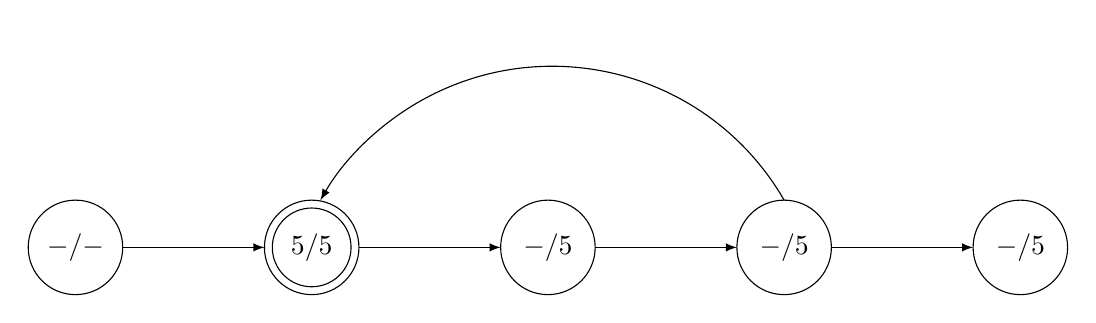
\begin{tikzpicture}
\draw (-4,0) node[draw, circle, minimum size=\noderadius] {$-/-$};
\draw[->, >=latex] (-4+\noderadiuspt,0) -- (-1-\noderadiuspt,0);
\draw (-1,0) node[draw, circle, minimum size=\noderadius] {$5/5$};
\draw (-1,0) node[draw, circle, minimum size=\noderadius-0.2cm] {};
\draw[->, >=latex] (-1+\noderadiuspt,0) -- (2-\noderadiuspt,0);
\draw (2,0) node[draw, circle, minimum size=\noderadius] {$-/5$};
\draw[->, >=latex] (2+\noderadiuspt,0) -- (5-\noderadiuspt,0);
\draw (5,0) node[draw, circle, minimum size=\noderadius] {$-/5$};
\draw[->, >=latex] (5+\noderadiuspt,0) -- (8-\noderadiuspt,0);
\draw (8,0) node[draw, circle, minimum size=\noderadius] {$-/5$};
\draw[->, >=latex] (5,\noderadius/2) arc ({\marginangle}:{180 - \marginangle}:3.4);
\end{tikzpicture}

% uda sie, wartosc MAP ze stanu 2 przeszla na 3 i 4
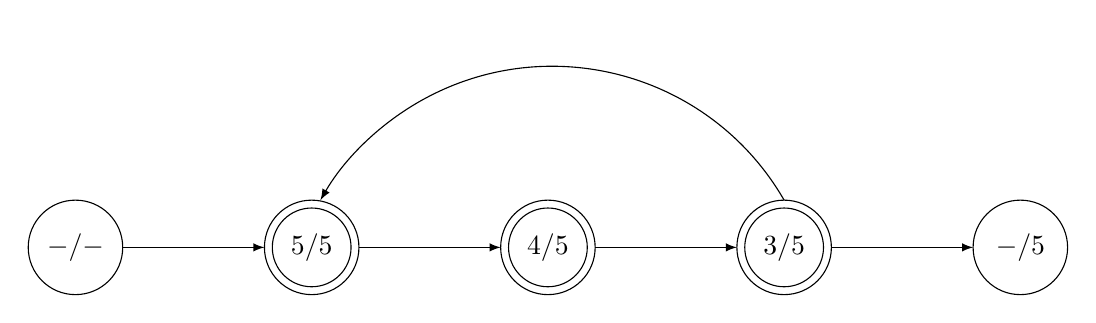
\begin{tikzpicture}
\draw (-4,0) node[draw, circle, minimum size=\noderadius] {$-/-$}; % null,null
\draw[->, >=latex] (-4+\noderadiuspt,0) -- (-1-\noderadiuspt,0);
\draw (-1,0) node[draw, circle, minimum size=\noderadius] {$5/5$}; % 5,5
\draw (-1,0) node[draw, circle, minimum size=\noderadius-0.2cm] {};
\draw[->, >=latex] (-1+\noderadiuspt,0) -- (2-\noderadiuspt,0);
\draw (2,0) node[draw, circle, minimum size=\noderadius] {$4/5$}; % 4,5
\draw (2,0) node[draw, circle, minimum size=\noderadius-0.2cm] {};
\draw[->, >=latex] (2+\noderadiuspt,0) -- (5-\noderadiuspt,0);
\draw (5,0) node[draw, circle, minimum size=\noderadius] {$3/5$}; % 3,5
\draw (5,0) node[draw, circle, minimum size=\noderadius-0.2cm] {};
\draw[->, >=latex] (5+\noderadiuspt,0) -- (8-\noderadiuspt,0);
\draw (8,0) node[draw, circle, minimum size=\noderadius] {$-/5$}; % null,5
\draw[->, >=latex] (5,\noderadius/2) arc ({\marginangle}:{180 - \marginangle}:3.4);
\end{tikzpicture}

% nie uda się -> kolejne stany akceptujące mają wiekszą wartość MAP, przez co poprzednia zostaje zapomniana
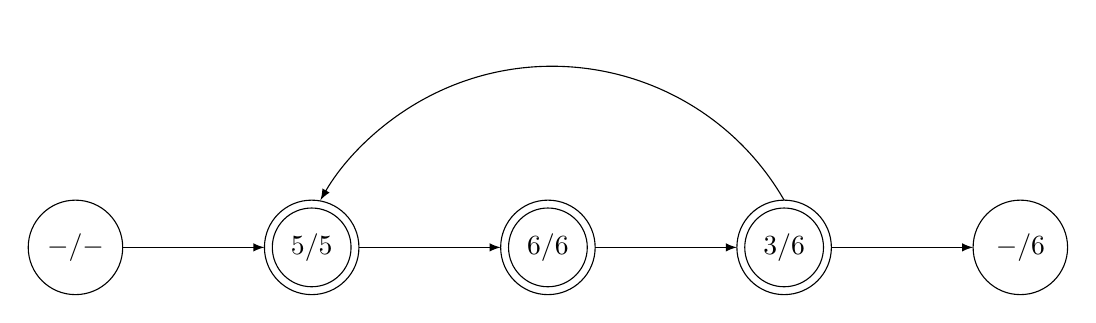
\begin{tikzpicture}
\draw (-4,0) node[draw, circle, minimum size=\noderadius] {$-/-$}; % null,null
\draw[->, >=latex] (-4+\noderadiuspt,0) -- (-1-\noderadiuspt,0);
\draw (-1,0) node[draw, circle, minimum size=\noderadius] {$5/5$}; % 5,5
\draw (-1,0) node[draw, circle, minimum size=\noderadius-0.2cm] {};
\draw[->, >=latex] (-1+\noderadiuspt,0) -- (2-\noderadiuspt,0);
\draw (2,0) node[draw, circle, minimum size=\noderadius] {$6/6$}; % 6,6
\draw (2,0) node[draw, circle, minimum size=\noderadius-0.2cm] {};
\draw[->, >=latex] (2+\noderadiuspt,0) -- (5-\noderadiuspt,0);
\draw (5,0) node[draw, circle, minimum size=\noderadius] {$3/6$}; % 3,6
\draw (5,0) node[draw, circle, minimum size=\noderadius-0.2cm] {};
\draw[->, >=latex] (5+\noderadiuspt,0) -- (8-\noderadiuspt,0);
\draw (8,0) node[draw, circle, minimum size=\noderadius] {$-/6$}; % null,6
\draw[->, >=latex] (5,\noderadius/2) arc ({\marginangle}:{180 - \marginangle}:3.4);
\end{tikzpicture}

% nie uda sie -> mimo poprawnej pętli, stan 3 nie jest źródłem wartości propagowanej dalej
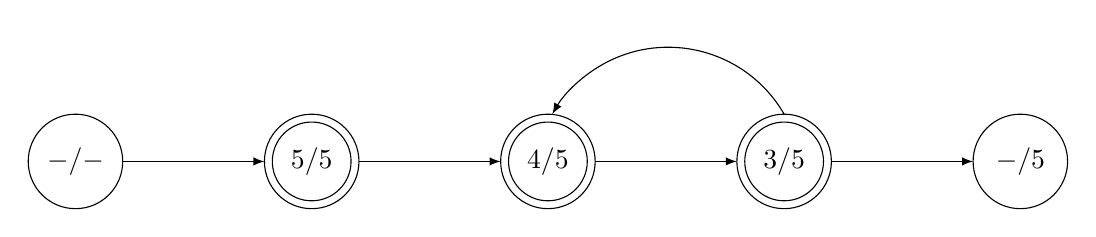
\begin{tikzpicture}
\draw (-4,0) node[draw, circle, minimum size=\noderadius] {$-/-$};
\draw[->, >=latex] (-4+\noderadiuspt,0) -- (-1-\noderadiuspt,0);
\draw (-1,0) node[draw, circle, minimum size=\noderadius] {$5/5$};
\draw (-1,0) node[draw, circle, minimum size=\noderadius-0.2cm] {};
\draw[->, >=latex] (-1+\noderadiuspt,0) -- (2-\noderadiuspt,0);
\draw (2,0) node[draw, circle, minimum size=\noderadius] {$4/5$};
\draw (2,0) node[draw, circle, minimum size=\noderadius-0.2cm] {};
\draw[->, >=latex] (2+\noderadiuspt,0) -- (5-\noderadiuspt,0);
\draw (5,0) node[draw, circle, minimum size=\noderadius] {$3/5$};
\draw (5,0) node[draw, circle, minimum size=\noderadius-0.2cm] {};
\draw[->, >=latex] (5+\noderadiuspt,0) -- (8-\noderadiuspt,0);
\draw (8,0) node[draw, circle, minimum size=\noderadius] {$-/5$};
\draw[->, >=latex] (5,\noderadius/2) arc ({\marginangle}:{180 - \marginangle}:1.7);
\end{tikzpicture}

\section{Ignore}

TODO

przestrzen stanow, automaty, automaty buchiego (przykladowe obrazki automatow z podanej formuly LTL, opis ze potrzebna negacja i szukanie spelnialnosci)
weryfikacja hardware i software
alogrytmy wykorzystywane w przeszukiwaniu i weryfikacji
co to i po co on-the-fly
Alvis, co to, po co

przejrzec publikacje profesora


w czesci implementacji:
opis weryfikowanego systemu


A time-optimal on-the-fly parallel algorithm for model checking of weak LTL properties, in: Formal Methods and Software Engineering
